\documentclass[conference, 12pt]{IEEEtran}
\usepackage{graphicx}
\usepackage{amsmath}
\usepackage{multirow}
\usepackage{hyperref}

\title{Graph Data Science for Author Domain Classification and Link Prediction}

\author{\IEEEauthorblockN{Basil Ali Khan, Hamza Ansari, Hayyan Khan} \\
\IEEEauthorblockA{Group 6\\ Graph Data Science, Spring 2025}}
\pagestyle{plain}
\begin{document}

\maketitle

\section{Introduction}
The source code used in this project is available on GitHub at the following link: 
\href{https://github.com/basil-ali-khan/Node_Classification_and_Link_Prediction_Using_Neo4}{GitHub Repository}.


\section{Data Preprocessing and Graph Modelling}
Data source: \cite{10.1162/qss_a_00163}\\
The dataset comprises academic publications represented as a 
heterogeneous graph consisting of Author, Paper, and Citation entities. 
Preprocessing was conducted using R, where the raw data was cleaned and 
missing values were handled.


The graph model was designed to represent the relationships between authors, papers, topics, journals, and publishers in the academic domain. The data was modeled as a heterogeneous graph in Neo4j, with the following node types and relationships:

\subsection{Nodes}
\begin{itemize}
    \item \textbf{Author}: Represents researchers or authors. Key properties include:
    \begin{itemize}
        \item \texttt{id}: Unique identifier for the author.
        \item \texttt{name}: Name of the author.
        \item \texttt{total\_citations}: Total number of citations received by the author's papers.
        \item \texttt{research\_domain}: The most researched topic by the author.
        \item \texttt{last\_collab\_year}: The most recent year of collaboration with other authors.
    \end{itemize}
    \item \textbf{Paper}: Represents academic papers. Key properties include:
    \begin{itemize}
        \item \texttt{id}: Unique identifier for the paper.
        \item \texttt{title}: Title of the paper.
        \item \texttt{year}: Year of publication.
        \item \texttt{citationCount}: Number of citations received by the paper.
    \end{itemize}
    \item \textbf{Topic}: Represents research topics. Key properties include:
    \begin{itemize}
        \item \texttt{id}: Unique identifier for the topic.
        \item \texttt{name}: Name of the topic.
    \end{itemize}
    \item \textbf{Journal}: Represents academic journals. Key properties include:
    \begin{itemize}
        \item \texttt{name}: Name of the journal.
    \end{itemize}
    \item \textbf{Publisher}: Represents publishers of journals. Key properties include:
    \begin{itemize}
        \item \texttt{name}: Name of the publisher.
    \end{itemize}
\end{itemize}

\subsection{Relationships}
\begin{itemize}
    \item \textbf{WROTE}: Connects an \texttt{Author} to a \texttt{Paper} they authored.
    \item \textbf{CO\_AUTHORED}: Connects two \texttt{Author} nodes who collaborated on the same paper. Includes:
    \begin{itemize}
        \item \texttt{collaboration\_year}: The year of collaboration.
    \end{itemize}
    \item \textbf{HAS\_TOPIC}: Connects a \texttt{Paper} to a \texttt{Topic} it addresses.
    \item \textbf{RESEARCHES}: Connects an \texttt{Author} to a \texttt{Topic} they have researched. Includes:
    \begin{itemize}
        \item \texttt{paper\_count}: Number of papers the author has written on the topic.
    \end{itemize}
    \item \textbf{SHARED\_TOPIC}: Connects two \texttt{Author} nodes who have researched the same topic. Includes:
    \begin{itemize}
        \item \texttt{shared\_topics}: Number of shared topics between the authors.
    \end{itemize}
    \item \textbf{SHARED\_JOURNAL}: Connects two \texttt{Author} nodes who have published in the same journal. Includes:
    \begin{itemize}
        \item \texttt{shared\_journals}: Number of shared journals between the authors.
    \end{itemize}
    \item \textbf{PUBLISHED\_IN}: Connects a \texttt{Paper} to the \texttt{Journal} it was published in.
    \item \textbf{PUBLISHED\_BY}: Connects a \texttt{Journal} to its \texttt{Publisher}.
    \item \textbf{CITES}: Connects one \texttt{Paper} to another paper it cites.
\end{itemize}

\begin{figure}[h]
    \centering
    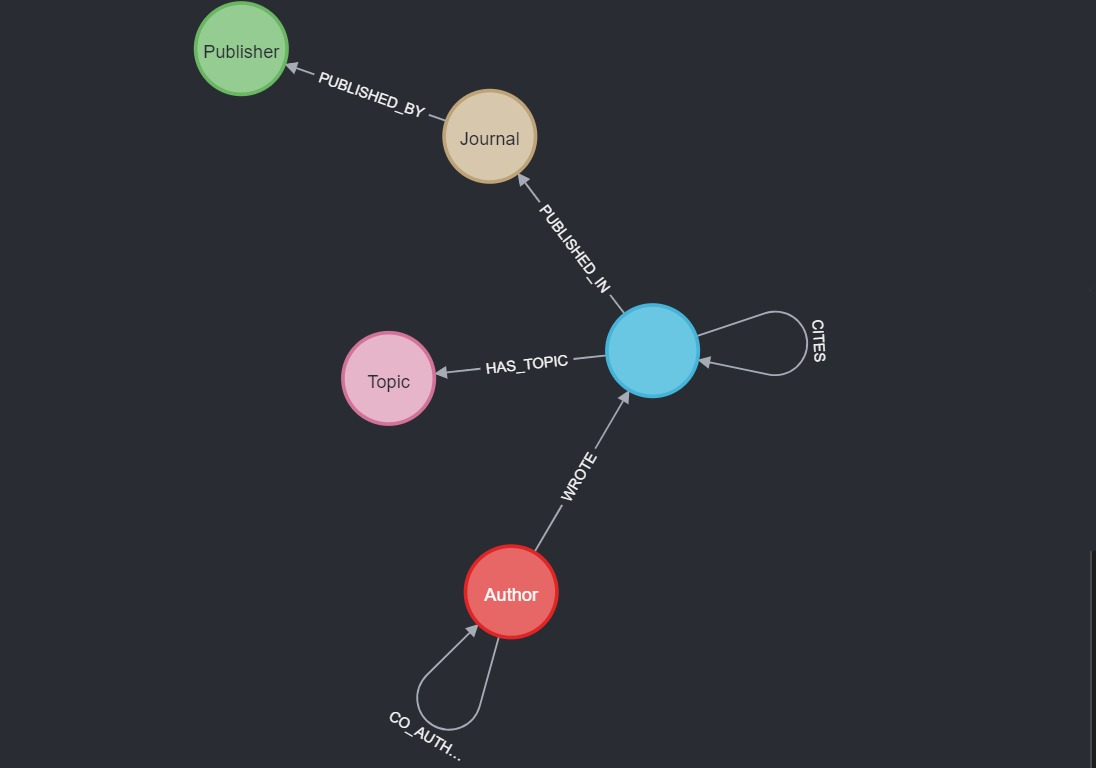
\includegraphics[width=\linewidth]{images/graph_model.jpg} 
    \caption{Data Model for the Graph}
    \label{fig:data_model}
\end{figure}

\subsection{Feature Engineering}
To enhance the graph model, additional features were computed:
\begin{itemize}
    \item \textbf{Total Citations}: The total number of citations received by an author's papers.
    \item \textbf{Research Domain}: The topic most frequently researched by an author.
    \item \textbf{Last Collaboration Year}: The most recent year an author collaborated with others.
\end{itemize}

\subsection{Neo4j Script For Graph Creation}
The Neo4j script to model the graph can be found in the github repository
in the $graph\_model\_creation\_script.txt$ file

\section{Methodology}

\subsection{Node Classification}

The node classification task aims to predict the research domain (\texttt{domain\_id}) of authors based on their co-authorship patterns and other features. We utilized the Neo4j Graph Data Science (GDS) library to train a machine learning model to classify authors into specific research domains. The authors were represented as nodes in a co-authorship graph, where edges between nodes (authors) represented collaborations (co-authorships) in academic papers.

\subsubsection{Graph Projection}
The first step in our methodology was to project the graph as follows:
\begin{itemize}
  \item \textbf{Nodes:} 
    \begin{itemize}
      \item \texttt{Author}: Represents an academic author. Each author node has a property \texttt{domain\_id} (the target classification label)
    \end{itemize}
  \item \textbf{Relationships:} 
    \begin{itemize}
      \item \texttt{CO\_AUTHOR}: Represents a collaboration between two authors on a paper.
    \end{itemize}
  \item \textbf{Label:} Authors with known research domains were tagged with the label \texttt{AuthorWithDomain} for the classification task. Authors without a known \texttt{domain\_id} were excluded from the node classification task.
\end{itemize}


\subsubsection{Feature Engineering}
To predict the \texttt{domain\_id}, we used the following features in the classification model:

\begin{itemize}
  \item \textbf{Louvain Community ID:} This feature was generated using the Louvain algorithm, which detects communities within the graph based on co-authorship patterns. Authors within the same community tend to have similar research topics, which makes this feature useful for domain classification.
  \item \textbf{Graph Embedding:} We generated graph embeddings using the Fast Random Projection (FastRP) algorithm. This technique transforms the graph structure into a vector space, capturing the local and global structure of the co-authorship network. Each author node was assigned an embedding vector representing its position within the network.
  \item \textbf{Domain ID (Target Property):} The target property for node classification was the \texttt{domain\_id}, which denotes the author's research domain. This was used to train the classification model.
\end{itemize}

These features were chosen because they provide both structural (co-authorship network) and domain-related information (community structure, embeddings) that can help in predicting the author's research domain.

\subsubsection{Machine Learning Model}
For node classification, we used the Random Forest classifier, which is robust to overfitting and effective for high-dimensional datasets like those encountered in graph-based tasks. The classifier was trained using the Neo4j Graph Data Science library, which provides built-in support for training machine learning models on graph data. The training process was configured as follows:

\begin{itemize}
  \item \textbf{Random Forest Classifier:} This ensemble method was chosen because it handles complex datasets well by combining multiple decision trees and averaging their outputs to improve accuracy and reduce overfitting.
  \item \textbf{5-Fold Cross-Validation:} To ensure generalization and prevent overfitting, we employed 5-fold cross-validation, splitting the data into 5 subsets. The model was trained on 4 subsets and validated on the remaining 1, rotating through all subsets.
  \item \textbf{Evaluation Metrics:} We evaluated the model's performance using several metrics, including:
    \begin{itemize}
      \item \textbf{F1-Weighted:} A harmonic mean of precision and recall, useful for imbalanced datasets.
      \item \textbf{Accuracy:} The proportion of correctly classified instances.
      \item \textbf{Out-of-Bag (OOB) Error:} This error metric provides an estimate of the classifier’s performance on unseen data.
    \end{itemize}
\end{itemize}

The model was trained on the graph, where the features (Louvain community ID, graph embeddings) were used to predict the \texttt{domain\_id} of each author.

\subsubsection{Model Training and Evaluation}
The training process was carried out in the Neo4j Graph Data Science environment using the following steps:

\begin{itemize}
  \item \textbf{Graph Projection:} A native projection was created for the \texttt{AuthorWithDomain} label using Cypher queries, ensuring that only the relevant nodes and relationships were included in the machine learning task.
  \item \textbf{Pipeline Construction:} The training pipeline was built using the Neo4j GDS library, including steps for feature extraction (Louvain, FastRP embedding), training the Random Forest model, and evaluating performance using cross-validation.
  \item \textbf{Model Training:} After defining the pipeline, the Random Forest model was trained using the features and the target \texttt{domain\_id}. The model parameters were tuned for optimal performance.
  \item \textbf{Model Evaluation:} The trained model's performance was evaluated using the metrics mentioned earlier, and the results were analyzed to identify areas of strength and potential improvement.
\end{itemize}

Once the model was trained, we used it to predict the \texttt{domain\_id} of authors who were not part of the training set, storing the predictions in a new property \texttt{predicted\_domain\_id} on each node.


\subsection{Link Prediction}
% Fill this in later by teammates

\section{Results}


\subsection{Node Classification Results}
The node classification model was trained to predict the \texttt{domain\_id} of authors in the co-authorship graph using a Random Forest classifier. After training and cross-validation, the following evaluation metrics were obtained from the Neo4j GDS pipeline:

\begin{itemize}
  \item \textbf{Test Accuracy:} 0.60
  \item \textbf{Test F1 Score:} 0.54
  \item \textbf{Out-of-Bag (OOB) Error:} 0.49
\end{itemize}

\begin{figure}[h]
    \centering
    \includegraphics[width=\linewidth]{images/NC_model_training_output.png} 
    \caption{Output after training pipeline}
    \label{fig:classification_metrics}
\end{figure}

These initial metrics reflect the model’s performance on a held-out validation set during training.

\subsubsection{Prediction Performance}
To further validate the model, we applied it to unseen nodes using the `predict.stream` procedure in GDS and compared the predicted domain labels with the ground truth labels. The following evaluation metrics were calculated based on the predictions:

\begin{itemize}
  \item \textbf{Accuracy:} 0.77
  \item \textbf{Precision:} 0.77
  \item \textbf{Recall:} 1.00
  \item \textbf{F1 Score:} 0.87
\end{itemize}

\begin{figure}[h]
    \centering
    \includegraphics[width=\linewidth]{images/NC_accuracy.png} % Replace with your image file
    \caption{Accuracy}
    \label{fig:accuracy}
\end{figure}

\begin{figure}[h]
    \centering
    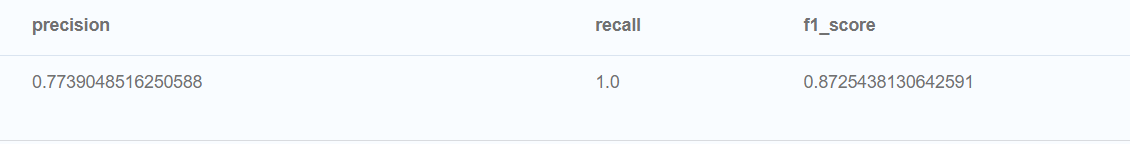
\includegraphics[width=\linewidth]{images/NC_precision_recall_f1score.png} % Replace with your image file
    \caption{Precision Recall and F1 Score}
    \label{fig:NC_Precision_Recall}
\end{figure}

The high recall value indicates that the classifier successfully predicted nearly all actual instances of each domain class. However, the slightly lower precision suggests that there were some false positives, indicating the need for improved feature representation or model tuning.


\subsection{Link Prediction Results}
% To be filled in by teammates working on link prediction.


\section{Discussion}

The node classification task yielded promising results, demonstrating that structural graph features like community membership and FastRP embeddings can reasonably predict an author's research domain. However, several limitations and areas for improvement were identified.

\subsection{Limitations and Challenges}
A key limitation was the quality of node embeddings. Several authors—particularly those with few or no co-authors—received zero or low-informative embedding vectors, which hindered classification accuracy. Additionally, the presence of interdisciplinary authors, who collaborate across multiple research domains, introduced ambiguity in both graph structure and labels. These factors contributed to misclassifications and highlight the need for more robust features beyond network structure.
\\Moreover, the model training itself was an extremely time consuming task, because of which we kept the embeddingDimension and numberOfDecisionTrees value low.

\subsection{Alternative Approaches}
Alternative graph embedding techniques, such as Node2Vec, could be explored to better capture node similarity in sparse or heterogeneous graphs. Additionally, incorporating non-structural node features—such as publication keywords, journal categories, or citation counts—could enrich the feature set and provide context where structural signals are weak. These features could be extracted using NLP techniques applied to paper titles or abstracts.

\subsection{Possible Extensions}
A natural extension would involve deploying Graph Neural Networks (GNNs), which can learn more expressive representations by aggregating features from neighborhood nodes. 
 Another promising direction is to use semi-supervised learning to infer domain labels for authors not included in the initial labeled set. This would expand the model’s applicability and improve generalization across the graph.

Overall, while the Random Forest classifier with FastRP embeddings performed well under certain conditions, integrating richer node features and leveraging advanced GNN-based methods could significantly enhance model robustness and accuracy in future work.


\bibliographystyle{IEEEtran}
\bibliography{references} % Add references.bib file for citations

\end{document}
